\chapter{Simulazioni e valutazione risultati}
\label{chap:sim_val}

\section{Organizzazione simulazioni}
La parte di realizzazione sperimentale del nostro progetto, è stata fatta tramite simulazioni con lo scopo di verificare il comportamento del nostro algoritmo e raccogliere dati per fare un'analisi più oggettiva delle sue prestazioni al variare delle condizioni. Per avere una sufficiente base statistica, abbiamo impostato nel file d'inizializzazione il numero di simulazioni a 20. Significa che per ogni configurazione il simulatore eseguirà venti simulazioni consecutive senza reimpostare il generatore di numeri casuali, in questo modo abbiamo ottenuto venti configurazioni di rete differenti per ogni configurazione. Per impostare il numero di ripetizioni da eseguire, abbiamo inserito nella sezione General di ogni file d'inizializzazione utilizzato, l'istruzione “repeat = 20”.

Le simulazioni sono state organizzate rispetto a due parametri principalmente: la densità di nodi e il raggio di trasmissione del BT. Come presentato nella \MySec{sec:modello_rete}, le densità studiate sono:
\begin{itemize}
	\item $d = 0.02 \, \dfrac{nodi}{m^{2}} $.
	\item $d = 0.01 \, \dfrac{nodi}{m^{2}} $.
	\item $d = 0.008 \, \dfrac{nodi}{m^{2}} $.
	\item $d = 0.001 \, \dfrac{nodi}{m^{2}} $.
	\item $d = 0.0005 \, \dfrac{nodi}{m^{2}} $.
	\item $d = 0.0001 \, \dfrac{nodi}{m^{2}} $.
\end{itemize}
E i valori del raggio $\rho$ sono:
\begin{itemize}
	\item $\rho$ = 15 m.
	\item $\rho$ = 50 m.
\end{itemize}
Le densità da $d=0.02\,nodi/m^2$ a $d=0.001\, nodi/m^2$ sono state pensate per simulare ambienti urbani che possono essere dal mediamente popolati al densamente popolati. Situazioni simili sono il caso di medie-grandi città o per le densità più elevate, situazioni di forte concentrazione di persone in un'area ristretta. Quest'ultimo caso può essere generato da una locale alta concentrazione abitativa come una serie di palazzi o condomini vicini tra loro, ma anche da motivazioni esterne come eventi che concentrano molte persone in uno stesso luogo. Le densità più piccole, $d=0.0005\, nodi/m^2$ e $d=0.0001\, nodi/m^2$ sono state pensate per studiare la scalabilità del sistema a fronte della dispersione dei nodi su una vasta area, ma anche per simulare situazioni urbanistiche tipiche di piccoli comuni, con un relativo basso numero di abitanti come ad esempio i piccoli paesi di campagna. Abbiamo quindi organizzato il processo di realizzazione sperimentale in modo da eseguire, per ogni densità, simulazioni per entrambi i raggi $\rho$ e collezionare dati per un'analisi a posteriori delle performance.

Il principale risultato che abbiamo voluto monitorare è stato la percentuale di diffusione dell'informazione al diminuire della densità, per studiare quali fossero i limiti di applicabilità in termini di efficienza del sistema e per avere un insieme di scenari in cui l'algoritmo da noi proposto presentasse buoni livelli di prestazioni. Parallelamente abbiamo anche raccolto dati sul tempo totale di trasmissione, inteso come l'istante di tempo in cui l'ultima trasmissione si è conclusa. Abbiamo scelto di raccogliere anche quest'ultimo dato perché abbiamo cercato di capire quali sono i tempi medi e massimi di diffusione del messaggio. Il motivo è stato di voler dare un corrispettivo valore temporale alla percentuale di nodi che l'algoritmo raggiunge. Da solo un valore di tempo massimo di trasmissione non è valutabile, poiché è molto dipendente dalla dispersione spaziale della rete; per come è costruita la rete non vi è garanzia che tutti i nodi siano connessi ad uno stesso grafo. Per questo motivo, il tempo totale di trasmissione deve essere analizzato in coppia con il valore percentuale di rete coperta durante quella specifica simulazione. In questo modo possiamo avere un'idea di come il tempo di propagazione evolva al variare della copertura e della densità della rete.
\bigskip

\subsection{Algoritmo Dynamic Fanout: funzionamento}
In questa sezione diamo una breve spiegazione sul funzionamento dell'algoritmo all'atto pratico dell'esecuzione. Presenteremo il suo comportamento descrivendo le tre principali configurazioni di lavoro. Faremo riferimento ai diagrammi di flusso in \MyAppendix{apx:diagrammi_fsa} durante la descrizione. Ricordiamo che i diagrammi rappresentano l'elenco di istruzioni della relativa situazione di lavoro. I tre principali momenti di lavoro sono i seguenti: standby, invio di un nuovo messaggio e Ricezione di un messaggio. Vi è anche un'insieme di istruzioni parallelo alle tre configurazioni, che viene eseguito sempre, in maniera periodica.
\bigskip

\noindent{\textbf{\textit{Standby}}}

Partiamo con la situazione di standby e si faccia riferimento al diagramma in \MyAppendix{apx:stb_fsa}. Quando il sistema si trova in una situazione di Standby, vuol dire che in quel momento non è impegnato in nessuna trasmissione nè ricezione. In questa situazione di lavoro il sistema, inizia nello stato di Standby del \acs{BLE}. All'occorrenza dell'esecuzione delle azioni periodiche, vengono eseguiti i rispettivi calcoli periodici e poi viene fatto un controllo se la batteria è sopra la soglia limite del 10\% e se il sistema non sia occupato. Ovviamente essendo in stato di Standby il sistema non è impegnato in nessuna attività e se vi è sufficiente batteria, il sistema passa in stato di Initiating, rimanendo in ascolto e aspettando eventuali comunicazioni sulla rete. Parallelamente, con in maniera ciclica e indipendente, verranno eseguire le azioni periodiche e ogni volta, dopo, verrà fatto il controllo sul livello di batteria. Qualora esso scenda sotto la soglia limite, il sistema verrà portato in stato di Standby e da li non si muoverà finché la batteria non verrà ricaricata. Le azioni periodiche vengono eseguite sempre anche quando il sistema in Standby per monitorare lo stato della rete e della batteria del dispositivo.

Indipendentemente dallo stato in cui il sistema si trova, Standby o Initiating, se il sistema riceve dall'utente il comando di inviare un nuovo messaggio, il dispositivo passa a eseguire le istruzioni della configurazione di invio messaggio. Viene lasciata la possibilità di inviare un messaggio dallo stato di Standby, anche se la batteria è inferiore al 10\%, perché negli scenari di lavoro ipotizzati, potrebbe rivelarsi comunque utile inviare un nuovo messaggio, anche se si potrebbe inficiare sull'autonomia del dispositivo. In tale situazione il sistema invierà solo una volta il messaggio e poi si riporterà da solo in stato di Standby. Nel caso invece il sistema si trovi in stato di Initiating e percepisca un nuovo messaggio sulla rete, si porta in configurazione di ricezione.
\bigskip

\noindent{\textbf{\textit{Azioni periodiche}}}

Sempre in riferimento a \MyAppendix{apx:stb_fsa}, descriviamo cosa trattano le azioni periodiche. Il sistema schedula ad intervalli regolari, un insieme di istruzioni da eseguire chiamate azioni periodiche. Queste azioni sono eseguite sempre, indipendentemente dalla situazione e dalla configurazione in cui il dispositivo sta operando. La periodicità è stata scelta di 30 secondi. Le azioni periodiche servono per aggiornare i parametri utilizzati dall'algoritmo di diffusione (\acs{DF} e \acs{AL}), in modo che dinamicamente si adattino all'ambiente esterno e allo stato attuale del dispositivo stesso. Dopo le operazioni di aggiornamento, viene anche fatto un controllo sul livello della batteria, come descritto per la configurazione di standby. Il controllo riguarda il livello della batteria e se il sistema rileva che la batteria è sopra la soglia limite (10\% come soglia limite), allora non interviene, ma nel caso sia sotto la soglia limite, viene segnalato e se il dispositivo non è impegnato il sistema viene portato in stato di Standby in cui rimarrà finché la batteria non tornerà sopra il 10\%. Questi controlli avvengono anche durante trasmissioni di scambio dati, ma in quel caso il sistema è occupato e si lascia terminare l'operazione, prima di portare il sistema in Standby. Non si vuole che una trasmissione già iniziata venga troncata a causa del controllo, poiché non vogliamo che vada a intralciare il processo di diffusione dell'informazione, ma può comunque agire tra una trasmissione e l'altra. Questo non grava troppo sull'autonomia in quanto il singolo scambio dati, per quanto grossa possa essere l'informazione, non rappresenta una grossa richiesta energetica. Anche quando la batteria è sotto la soglia limite e il sistema è in stato di Standby, i controlli, grazie alla loro esigua richiesta energetica, sono sempre effettuati per riabilitare il sistema al lavoro attivo qualora la batteria venga ricaricata e torni sopra soglia. Una parte dei controlli periodici è già stata inserita e rappresentati nel diagramma di flusso della configurazione di standby, per dare una semplice idea di quale sia il compito di questi controlli, ma non sono vincolati a nessuna configurazione. Esse restano organizzate ed eseguite in maniera indipendente. Per quanto riguarda la sola parte di simulazione, abbiamo inserito nelle azioni periodiche anche il decremento della batteria dei dispositivi, per simulare l'uso del dispositivo da parte dell'utente. Il decremento è piccolo per indicare il consumo medio in idle. Per le trasmissioni completate invece, vi è un decremento più grande dovuto alla grandezza dell'informazione.
\bigskip

\noindent{\textbf{\textit{Invio di un messaggio}}}

Quando è necessario inviare un nuovo messaggio, che esso sia stato ricevuto dalla rete oppure venga inviato dall'utente, il sistema entra in configurazione di invio. Si faccia riferimento al diagramma all'\MyAppendix{apx:invio_fsa}. Appena entrato in questa modalità, il sistema controlla di eseguire una transizione di stato corretta, quindi se non era già in stato di Standby, si porta in stato di Standby. Poi vengono inizializzati i contatori di trasmissioni e di \acs{AE}. A questo punto può entrare in stato di Advertising e iniziare le operazioni per l'invio. Viene incrementato di uno il contatore degli AE e poi il sistema esegue l'\acs{AE} vero e proprio. Durante l'\acs{AE} il sistema trasmette pacchetti di tipo "advertising indiretto" (ADV\_IND \cite{BT-CoreSpec4.0}). Dopo di che si mette in ascolto, aspettando eventuali risposte e viene fatto partire il timeout. Se il timeout scade e nessuna richiesta di connessione è arrivata al dispositivo, esso controlla se il $\textit{AE counter}$ è minore dell'AL. In caso positivo, vuol dire che nessuno è più interessato e quindi viene riportato il sistema in configurazione di standby. In caso negativo invece, il sistema ricomincia tutto il processo di advertising. Nel caso invece che, prima dello scadere del timeout, arrivi una richiesta di connessione (CONN\_REQ \cite{BT-CoreSpec4.0}), il sistema procede a segnalare che è occupato in una trasmissione, così da evitare interruzioni dai controlli di sistema, e poi entra in stato di Connection col ruolo di Slave. Quando il nodo col ruolo di Master invia la richiesta id \textit{pool}, inizia il vero e proprio \acf{CE}, in cui il sistema trasmette al richiedente tutta l'informazione. Al termine del \acs{CE}, viene incrementato il contatore di trasmissioni effettuate, viene decrementato il livello della batteria a causa della trasmissione appena effettuata, il sistema segnala di non essere più occupato, passa in stato di Standby e controlla che se ha raggiunto il limite di trasmissioni imposto dal DF. In caso affermativo, il sistema ha raggiunto la sua quota di lavoro e può tornare in configurazione di standby, mentre in caso contrario, il sistema si riporta in stato di Advertising pronto a ricominciare.
\bigskip

\noindent{\textbf{\textit{Ricezione di un messaggio}}}

Quando il dispositivo rileva che uno o più nodi stanno diffondendo informazioni che il sistema non ha ancora ricevuto, esso entra in configurazione di ricezione di un messaggio, descritto dal diagramma in \MyAppendix{apx:ricevi_fsa}. Questa configurazione è accessibile solo da uno stato di ascolto, ma comunque viene controllato come prima cosa che il sistema sia nel corretto stato. Se non si trova in stato di Initiating, si porta prima in stato di Standby e poi in stato di Initiating. A questo punto il sistema è pronto alla connettersi, quindi risponderà al primo pacchetto di advertising (ADV\_IND \cite{BT-CoreSpec4.0}) che riceve, inviando a sua volta una richiesta di connessione (CONN\_REQ \cite{BT-CoreSpec4.0}). Dopo di che, il sistema si segna occupato e entra in stato di Connection col ruolo di Master. A questo punto invia la sua richiesta di \textit{pool} e lancia il timeout. Il sistema non sa ancora se il dispositivo mittente ha accettato la sua connessione. L'unica cosa che può fare dopo aver inviato la richiesta di pool, è aspettare. Se il timeout scade e non è stata ricevuta nessuna informazione, vuol dire che il mittente non ha accettato la richiesta di connessione oppure era già impegnato in un altra trasmissione. Capendo di non essere stato scelto per la trasmissione, il sistema si dichiara non occupato e si riporta in stato di Initiating in ascolto, pronto a ricominciare. Nel caso invece la richiesta di connessione venga accetta, in risposta alla richiesta di \textit{pool}, inizierà il \acs{CE} e il dispositivo advertiser invierà l'informazione. Una volta terminato il \acs{CE}, viene decrementato il livello della batteria a causa della trasmissione appena effettuata, il sistema si dice non più occupato e si prepara ad entrare in configurazione di invio per diffondere a sua volta l'informazione.
\bigskip

\section{Valutazione risultati}
Dopo aver terminato le simulazioni, abbiamo raccolto i dati ed eseguito analisi su di essi. I parametri che abbiamo monitorato come risultati, a fronte dell'invio di un singolo messaggio sono stati:
\begin{itemize}
	\item Copertura: percentuale di contagio che il messaggio ha raggiunto.
	\item Tempo totale di trasmissione: tempo totale impiegato per raggiungere tale copertura di rete.
\end{itemize}
Grazie alle funzionalità offerte dal framework di simulazione OMNeT++, è stato possibile raccogliere i dati in maniera efficiente. Con una manipolazione dei dati appena raccolti, il framework è stato in grado di fornirci il valor medio, la varianza, la deviazione standard e anche l'intervallo di confidenza al 95\%. Abbiamo anche estratto dai dati raccolti, gli stessi indici tramite un foglio di calcolo Excel, in modo da poter validare ed eventualmente correggere eventuali errori o approssimazioni del software di simulazione.

Prima di parlare dei singoli risultati, ripetiamo alcuni aspetti che hanno caratterizzato l'algoritmo, i modelli e la simulazione stessa. Per avere una maggior variabilità nella simulazione, abbiamo assegnato molti valori di parametri tramite l'uso di generatori casuali, come ad esempio la disposizione dei nodi nella rete, il livello di batteria iniziale di ogni dispositivo e, per ogni ripetizione, la scelta del nodo che possiede l'informazione da divulgare e che inizierà la diffusione. Per ogni densità, sono stati simulati i due range $\rho$ scelti, $\rho=15m$ e $\rho=50m$, e poi è stata fatta la media tra i due. Inoltre la diversità di prestazioni dovuta alla differenza di raggio $\rho$ utilizzato è elevata. Questi aspetti saranno ripresi quando illustreremo i risultati ottenuti.

Il primo parametro che presentiamo è quello della percentuale di rete contagiata dal messaggio, la \textbf{\textit{copertura}}. In \myFig{fig:copertura} sono riportati su grafico i valori medi dei dati raccolti relativi alla copertura raggiunta dal messaggio, per ogni densità simulata. Per ogni curva abbiamo anche riportato sul grafico, il suo intervallo di confidenza al 95\%, per comprendere la distribuzione attorno ai valori medi. La prima cosa che si nota è che per le densità $d=0.02\, nodi/m^2$, $d=0.01\, nodi/m^2$ e $d=0.008\, nodi/m^2$ la percentuale di contagio è intorno al 100\% ed è indicativo di un'ottima efficienza prestazionale della soluzione da noi proposta in ambienti densamente popolati o in momenti di alta concentrazione urbana per motivi particolari. Per queste tre densità molto alte entrambi i raggi $\rho$ hanno dato ottimi valori. Le tre densità più piccole invece hanno evidenziato i limiti di operabilità del sistema. Per la densità $d=0.001\, nodi/m^2$, abbiamo ottenuto ancora degli ottimi valori in termini di copertura, ma in questo caso, il raggio $\rho=15m$ ha cominciato a evidenziare problemi nello stabilire collegamenti tra i nodi e quindi raggiungere un'ottima copertura. Per questo motivo abbiamo ottenuto un intervallo di confidenza già ben più ampio rispetto alle tre casistiche precedenti nelle quali era pressoché nullo o molto piccolo. Nel complesso rimane comunque stabile in un intorno del 90\% al crescere del numero dei nodi nella rete.
\bigskip
\begin{figure}[t]
	\centering
	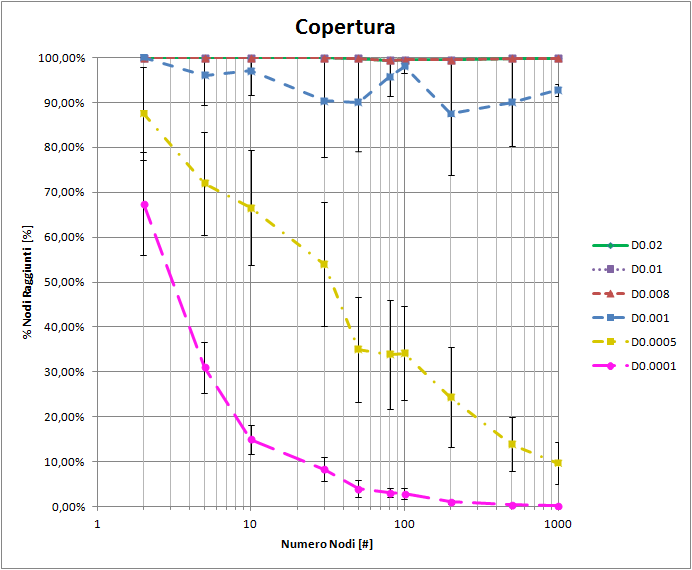
\includegraphics[width=0.9\linewidth]{Images/risultati/copertura}
	\caption[Copertura]{Grafico della copertura della rete.}
	\label{fig:copertura}
\end{figure}

Poi abbiamo la curva della densità $d=0.0005\, nodi/m^2$. Questo valore di densità, rispetto al precedente, presenta un andamento decrescente, al crescere del numero di nodi. Già a questo livello di densità, abbiamo riscontrato che al crescere della rete, aumenta la probabilità che si formino sottoreti isolate che causano solo una diffusione parziale del messaggio. Rispetto alla densità precedente che era il doppio, abbiamo avuto un forte deterioramento nella copertura della rete e un più ampio intervallo di confidenza. Con questo valore di densità, si ha che al crescere del numero di nodi, essi comincino ad essere troppo diradati nella rete e nel complesso si vengano a creare sottoreti sempre più piccole col crescere del numero di nodi. Con le ipotesi fatte, non vi è modo per l'algoritmo di eludere o superare quest'ostacolo. Nonostante quest'andamento decrescente, possiamo vedere che con mille nodi nella rete, il sistema sarebbe in grado di coprire una porzione di rete intorno al 10\%; per questo motivo la densità $d=0.0005\, nodi/m^2$ può essere considerata un limite inferiore di operatività. Infine l'ultima densità $d=0.0001\, nodi/m^2$ si dimostra essere oltre le possibilità operative del sistema, infatti, mostra un degrado prestazionale forte già con reti piccole composte di soli dieci nodi.
Dalle nostre simulazioni è emerso che il sistema è in grado di gestire e operare a livelli ottimi, copertura intorno al 90\% circa, fino a densità $d=0.001\, nodi/m^2$ ma può operare, se pur con un degrado prestazionale linearmente dipendente dalla grandezza della rete, anche fino a una densità minima di $d=0.0005\, nodi/m^2$.

\begin{figure}[t]
	\centering
	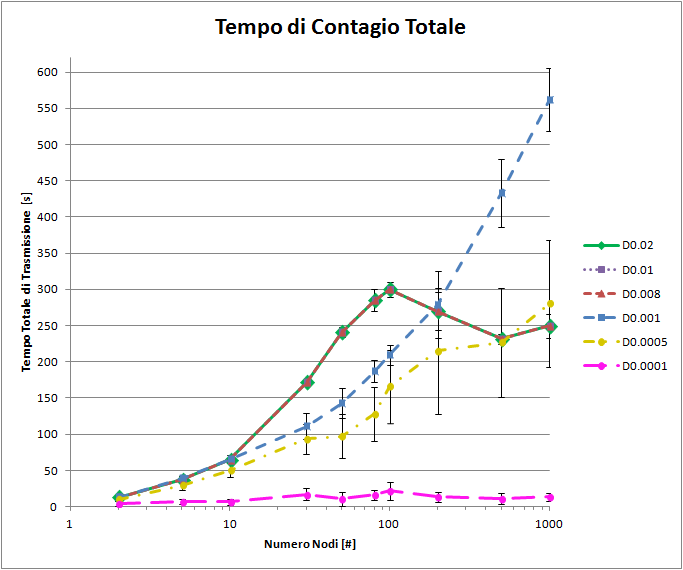
\includegraphics[width=0.9\linewidth]{Images/risultati/tempo_totale}
	\caption[Tempo totale di trasmissione]{Grafico del tempo totale di trasmissione.}
	\label{fig:tempo_totale}
\end{figure}
In \myFig{fig:tempo_totale} riportiamo i risultati riguardanti il \textbf{\textit{tempo totale di trasmissione}}, tempo che l'algoritmo ha impiegato per completare l'ultima trasmissione di contagio a lui possibile. Dalle nostre analisi è risultato che per densità basse come $d=0.02\, nodi/m^2$, $d=0.01\, nodi/m^2$ e $d=0.008\, nodi/m^2$, l'alta vicinanza a permesso di contenere il tempo necessario e dopo un picco in corrispondenza di cento nodi, esso diminuisce pur garantendo una copertura totale o quasi. Questo grazie all'alta ridondanza di collegamenti creatasi dalla vicinanza dei nodi; in questo modo la rete stessa riesce a evitare la formazione di colli di bottiglia tra gruppi di nodi. Per $d=0.001\, nodi/m^2$ invece, abbiamo un andamento crescente col numero di nodi, anche se in \myFig{fig:copertura} si vede come resti sempre vicino alla copertura totale.  In questo caso abbiamo un andamento di tipo quadratico, al crescere del numero di nodi nella rete. Già passando da $d=0.008\, nodi/m^2$ a $d=0.001\, nodi/m^2$ si può notare come cambi il tempo necessario all'algoritmo per raggiungere la sua massima copertura. Infine, le densità d=0.0005 e d=0.0001 presentano curve inferiori alle precedenti ma vanno lette in combinazione con i risultati mostrati in \myFig{fig:copertura}. 
Notiamo che l'andamento, almeno per la curva $d=0.0005\, nodi/m^2$, riamane di tipo quadratico, indice di una rete sempre più diradata nella quale si perdono sempre più i collegamenti ridondanti tra i nodi e compaiono sempre più sottoreti e singoli collegamenti tra essi, che sono il punto debole dell'algoritmo. Se al crescere del numero di nodi, la percentuale di rete coperta diminuisce, significa che il sistema esegue sempre meno trasmissioni, per questa ragione le curve per $d=0.0005\, nodi/m^2$ e $d=0.0001\, nodi/m^2$ sono inferiori alle altre. Per la curva di densità più bassa $d=0.0001\, nodi/m^2$, possiamo solo da dire che conferma i dati rilevati della copertura. L'impossibilità eseguire trasmissioni a causa di una rete troppo sparsa, fa sì che l'algoritmo perda efficacia e si fermi dopo pochi secondi di operatività.

Per valutare meglio l'efficacia della propagazione, abbiamo anche analizzato un \textit{\textbf{fattore di efficienza}}: il rapporto tra la copertura raggiunta, in termini di numero di nodi, e il tempo impiegato per raggiungerla. In \myFig{fig:fattorediefficienza_log} riportiamo i risultati su grafico. Dal grafico si nota come tutte le densità tra $d=0.02\, nodi/m^2$ a $d=0.001\, nodi/m^2$ siano molto simili in termini di efficienza. L'estrema vicinanza tra i nodi per $d=0.02\, nodi/m^2$, rende l'algoritmo molto efficace, ma anche scendendo fino a $d=0.001\, nodi/m^2$ l'efficienza dell'algoritmo rimane buona e l'andamento rimane lo stesso delle densità più alte. Per le due densità limite invece si nota come l'efficienza per la $d=0.0005\, nodi/m^2$ fatichi ad aumentare all'aumentare del numero di nodi, mentre per la $d=0.0001\, nodi/m^2$ si noti come continui a decrescere, fatta eccezione per qualche piccolo picco e per il valore superiore per $n=2$. Quest'ultimo fatto è dovuto a una scelta di progettazione, per agevolare l'analisi dei dati. Quando il primo nodo è inizializzato col messaggio da inviare, il sistema registra il tempo di consegna come l'istante del primo contagio che è sicuramente inferiore al tempo necessario per contagiare l'altro nodo, in una rete formata da due soli nodi. Per questo motivo, per reti piccole risulta avere un'efficienza più alta. All'aumentare della grandezza della rete la curva per $d=0.0001\, nodi/m^2$ si stabilizza e non presenta più il problema, rappresentando il corretto andamento.
\begin{figure}[t]
	\centering
	\includegraphics[width=0.9\linewidth]{"Images/risultati/fattore di efficienza_log"}
	\caption[Fattore di Efficienza]{Grafico del fattore di efficienza}
	\label{fig:fattorediefficienza_log}
\end{figure}

Dopo l'analisi dei dati raccolti, è difficile poter dire con che legge si comporta il nostro algoritmo, per vari motivi. Il primo tra tutti è che non abbiamo sempre una situazione in cui ogni nodo sia connesso in un unico grafo. Le diverse densità possono creare più sottografi isolati senza la possibilità che questi ultimi possano comunicare. Un altro fattore importante è che i nodi del grafo sono dispositivi con una batteria e l'energia a disposizione si consuma nel tempo. Nodi in posizioni critiche della rete possono esaurire la batteria e così escludere parte della rete. Sul fattore batteria sono calibrati i parametri del sistema, e i limiti di trasmissione. Un nodo con limiti di trasmissione bassi, potrebbe completare il suo lavoro di trasmissione, ma verso una zona di rete già abbastanza informata e non in una zona di rete in cui l'informazione non è ancora arrivata. Un altro fattore molto importante e influente, è il metodo (o i metodi) di terminazione che si è scelto di utilizzare. Differenti metodi con differenti criteri possono portare ad avere prestazioni molto differenti.

In condizioni ideali, tutti i nodi connessi in un unico grafo e batteria infinita per tutti i dispositivi, come presentato in \cite{gossip2000-comp} e in \cite{schindel2004-epidemicAlg}, gli algoritmi di rumor mongering con strategia di diffusione push\&pull hanno queste caratteristiche:
\begin{itemize}
	\item L'informazione viene diffusa a tutti dopo $ O\left( \ln \mathit{n} \right)  $ cicli.
	\item La copertura completa richiede almeno $ O\left( \mathit{n}\cdot\log \log \mathit{n} \right)  $ trasmissioni/messaggi.
\end{itemize}
Con \textit{n} il numero di nodi della rete. Per gli algoritmi di rumor mongering di tipo "\textit{address-indipendent}", le complessità appena elencate sono completamente indipendenti dal modo in cui vengono scegli i nodi con cui comunicare e le distribuzioni di probabilità con cui i nodi vengono scelti. Gli algoritmi di tipo "\textit{address-indipendent}" sono algoritmi che, ad ogni iterazione, non dipendono dalla posizione e/o dall'indirizzo dei nodi vicini, ma solo dal numero di nodi vicini. Per questo motivo, questi algoritmi lavorano allo stesso modo sia se hanno una visione completa della rete sia se hanno una visione parziale della rete, l'importante è che siano "\textit{address-indipendent}".

Aspetti che non sono stati considerati in questo studio e che possono avere un impatto sulle prestazioni sono: la mobilità dei nodi e una distribuzione dei nodi nell'area non più totalmente uniforme, ma con una logica più vicina al centro abitativo. Le zone abitative sono costruite vicino ad altre già presenti e non in maniera uniforme su un determinato territorio. La mobilità può creare situazioni riconducibili ai veri contagi epidemici. Un nodo a conoscenza di un'informazione può spostarsi in una zona, anche lontana dal punto di partenza, dove l'informazione sarebbe impossibilitata ad arrivare e iniziarne la diffusione. Questo porterebbe a ridurre i problemi generati dalla bassa densità e dalla conseguente formazione di sottoreti isolate.